\section{Architecture Description}

The first problem to solve is the \textbf{complexity} of the \textbf{operations}. In fact, the linear interpolation requires \textbf{multiplications} and \textbf{divisions}, whose circuits aren't trivial. But in this case the factor interpolation is fixed to $4$, and is a \textbf{power of two}. So is possible for example to exploit the \textbf{shift operation} in base two, to do the division by powers of two in a zero complexity way.

All the \textbf{simplifications} made in the calculation of all outputs are described below:

\[OUT_i = (y_{n+1} - y_n)\frac{i}{4} + y_n = y_{n+1} \frac{i}{4} - y_n \frac{i}{4} + y_n\] 
\[OUT_0 = y_{n+1} \frac{0}{4} - y_n \frac{0}{4} + y_n = y_n\] 
\[OUT_1 = y_{n+1} \frac{1}{4} - y_n \frac{1}{4} + y_n = y_{n+1} \frac{1}{4} + y_n \frac{3}{4} =  y_{n+1} \frac{1}{4} + y_n \frac{2}{4} + y_n \frac{1}{4} = y_{n+1} \frac{1}{4} + y_n \frac{1}{2} + y_n \frac{1}{4}\]
\[OUT_2 = y_{n+1} \frac{2}{4} - y_n \frac{2}{4} + y_n = y_{n+1} \frac{2}{4} + y_n \frac{2}{4} = y_{n+1} \frac{1}{2} + y_n \frac{1}{2}\] 
\[OUT_2 = y_{n+1} \frac{3}{4} - y_n \frac{3}{4} + y_n = y_{n+1} \frac{3}{4} + y_n \frac{1}{4} =  y_{n+1} \frac{1}{4} + y_{n+1} \frac{2}{4} + y_n \frac{1}{4} = y_{n+1} \frac{1}{4} + y_{n+1} \frac{1}{2} + y_n \frac{1}{4}\]

So in conclusion the equations that have to be implemented are:

\[OUT_0 =  y_n\] 
\[OUT_1 = \frac{y_{n+1}}{4} + \frac{y_n}{2} + \frac{y_n}{4}\]
\[OUT_2 = \frac{y_{n+1}}{2} + \frac{y_n}{2}\] 
\[OUT_2 = \frac{y_{n+1}}{4} + \frac{y_{n+1}}{2} + \frac{y_n}{4}\]

It's clear from the equations above that:

\begin{itemize}
    \item There are \textbf{no subtractions}, but only summations, so it is possible to use \textbf{unsigned signals} that can be summed by a Ripple Carry Adder.   
    \item There are \textbf{no multiplications}, but only divisions by powers of two. The signals are unsigned, so they can be implemented by \textbf{bit a bit right shifts}.
\end{itemize}

Using integer signals and divisions that ignores reminder, the results will have some \textbf{error} compared to the original formula. But this is an acceptable error, considering the huge benefits obtained in terms of circuit complexity.

\newpage

\subsection{Block Diagram}

An high level representation of the the circuit is the following:

\begin{figure}[H]
    \centering
    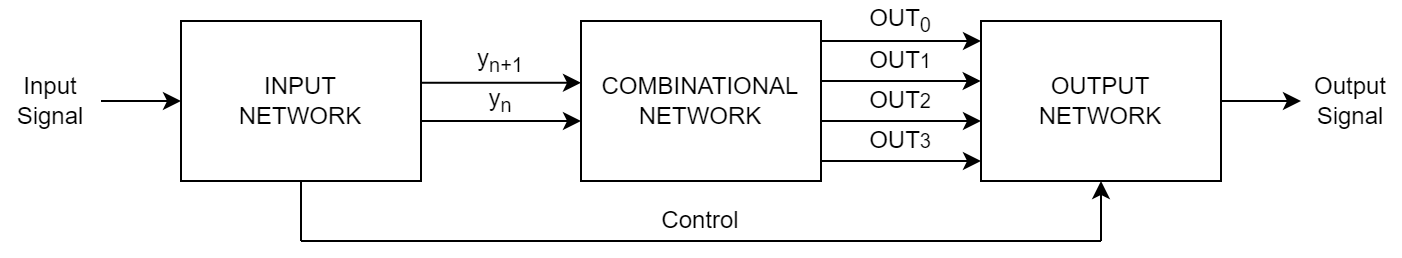
\includegraphics[width=1\textwidth]{img/Chapter2/BlockDiagram.png}
    \caption{Block Diagram}
    \label{fig:BlockDiagram}
\end{figure}

Every block will be analized, starting from the combinational network that performs the calculation of the output signals.

\subsection{Combinational Network}

The combinational network is at the heart of the circuit. Given two signals in input, it provides \textbf{all four interpolated signals}:

\begin{figure}[H]
    \centering
    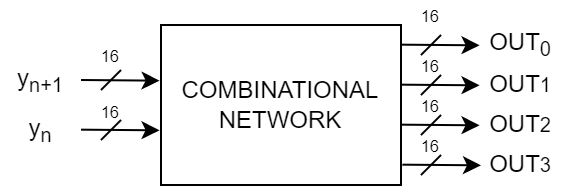
\includegraphics[width=0.6\textwidth]{img/Chapter2/CombinationalIO.png}
    \caption{Combinational Network I/O Ports}
    \label{fig:CNIO}
\end{figure}

The calculations is divided into two parts:

\begin{enumerate}
    \item It compute the \textbf{four signals needed} throw bit a bit shifts ($\frac{y_{n+1}}{4}, \frac{y_{n+1}}{2}, \frac{y_n}{4}, \frac{y_n}{2}$).
    \item It combine the signals obtained with a set of Ripple Carry Adders, to compute the \textbf{final results}.
\end{enumerate}

\newpage

The second point is implemented in this way:

\begin{figure}[H]
    \centering
    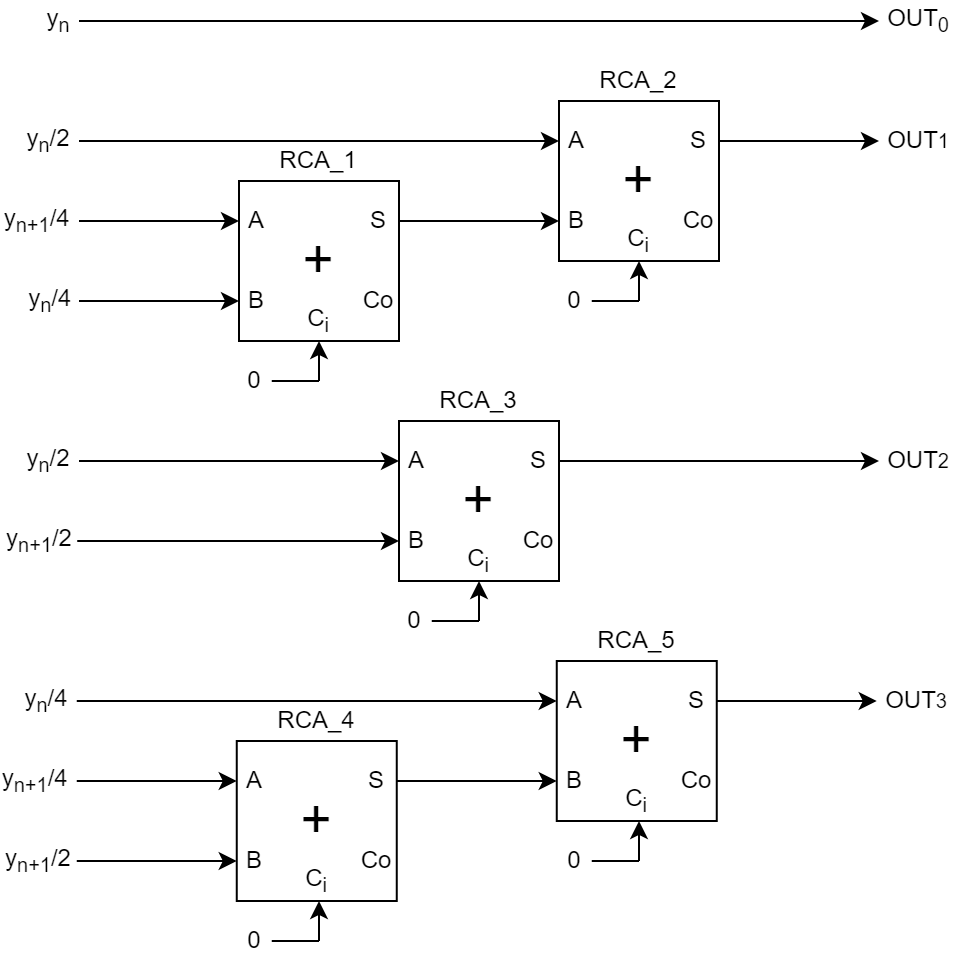
\includegraphics[width=0.6\textwidth]{img/Chapter2/CombinationalStructure.png}
    \caption{Output Signals Calculation}
    \label{fig:OutputSignalsCalc}
\end{figure}

So \textbf{five Ripple Carry Adders} are needed.

\subsubsection{The Synchronization Problem}

Before moving to the study of input and output blocks, it is necessary to consider that the frequency with which the output signals have to be produced is \textbf{four time greater} the input signals arrival frequency.

In order to evaluate the \textbf{timing requirements} of the circuit, registers after input and before output are needed (to have always a \textbf{register-logic-register structure}). So it's clear that the output register has to be updated more frequently than the one in input.

The possible solutions to this problem are two:

\begin{itemize}
    \item Implement \textbf{two different clock domains}, one with a period of $T$ and one of $\frac{T}{4}$.
    \item Implement only the fastest clock (the one with a period of $\frac{T}{4}$), and exploit the \textbf{input register enabler port} to memorize a new signal only once every four clock cycles.  
\end{itemize}

It's clear that the first solution offers the best performance, but at very high cost in terms of complexity. So the second solution has been chosen, that as before in the calculation of the output signals, is the \textbf{best trade-off} between performance and design complexity.

Now will be described how this solution has been implemented in the input network.

\subsection{Input Network}

The main purpose of this network is to \textbf{receive} and \textbf{memorize} every period $T$ the \textbf{new signal}, and to \textbf{maintain it stable} for the combinational network. Moreover even the \textbf{second last input} must also be kept stable, because it is required for the interpolation as well.

To do that \textbf{two registers}, composed by 16 \textbf{D Flip Flop}, have been used. The first register (named \textit{REG\_NI}) take in input the \textbf{receiving signal}. The output of this register provides the signal $y_{n+1}$ to the combinational network. Also it goes in input to a second register (named \textit{REG\_OI}). This second register provides to the combinational network the signal $y_n$. In fact, when the clock arrives \textit{REG\_NI} memorizes the new signal from the outside, and \textit{REG\_OI} memorizes the previous value contained in \textit{REG\_NI}.

The network described above looks like this:

\begin{figure}[H]
    \centering
    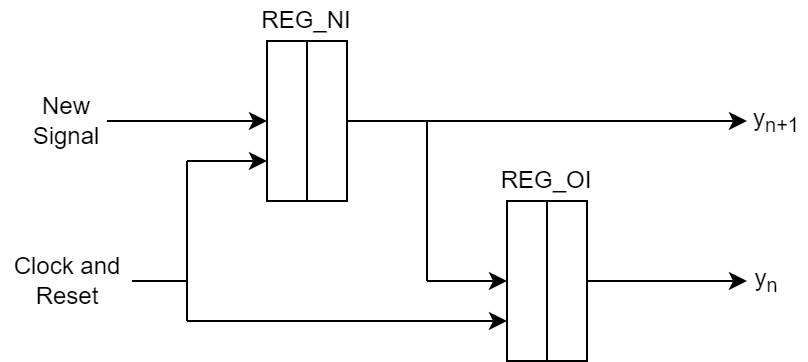
\includegraphics[width=0.5\textwidth]{img/Chapter2/InputNetwork1.png}
    \caption{Input Network Registers}
    \label{fig:InputNetwork1}
\end{figure}

In order to implement the \textbf{synchronization problem solution} (section 2.2.1) is necessary to set the registers enabler port to one every four clock cycle. To do that a \textbf{2 bit counter} has been implemented; it counts from 0 to 3, increasing its value of one \textbf{every clock cycle}. Assuming that a new signal arrives when the output of counter is 0, the enabler has to be one in the previous cycle, so when the counter output is 3 ($|11|_2$ in base 2). Therefore, the counter output goes in input to an \textbf{AND port}, whose output becomes the \textbf{enabler line} for the two input registers.

The resulting network is as follows:

\begin{figure}[H]
    \centering
    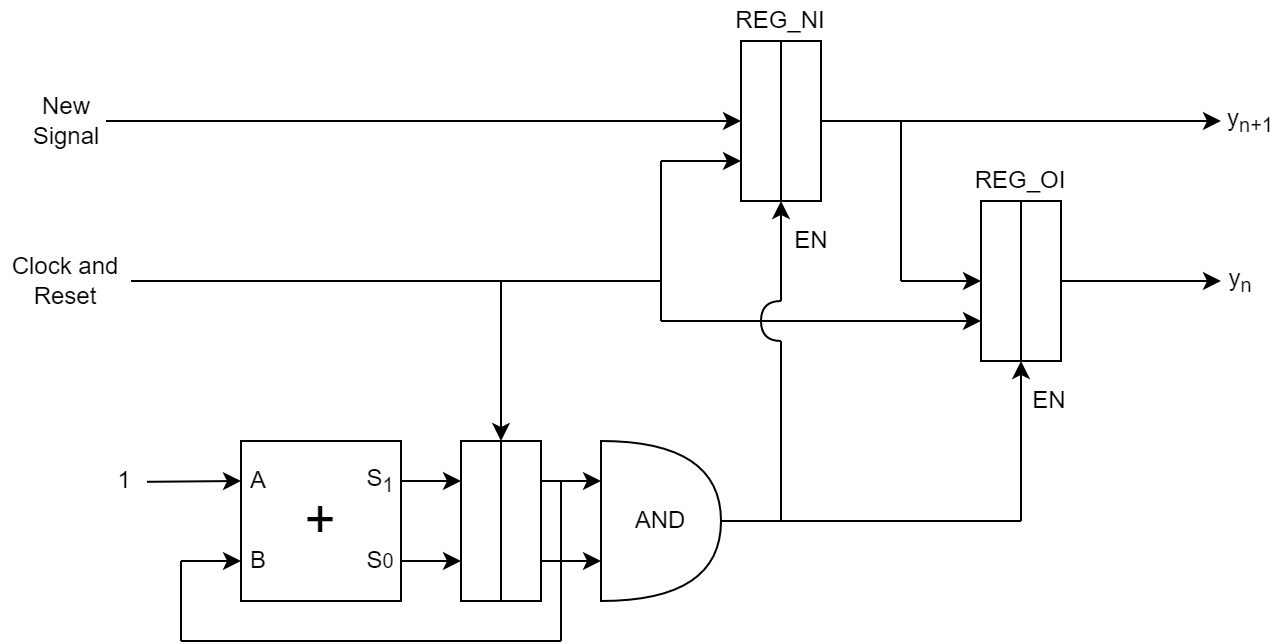
\includegraphics[width=0.65\textwidth]{img/Chapter2/InputNetwork2.png}
    \caption{Total Input Network}
    \label{fig:InputNetwork2}
\end{figure}

So \textbf{one Ripple Carry Adder}, \textbf{three Registers} and \textbf{an And Port} are needed.

\subsection{Output Network}

The last network of the circuit has to \textbf{output one at a time} the four signals calculated by the combinatorial network. 

To do that a \textbf{multiplexer} has been used. It take in input the four signals resulting from the combinational network and provides them one at time. The output of multiplexer is controlled by the \textbf{counter} of the \textbf{input network}, whose output is exactly a line that change from 0 to 3 every clock cycle.

The output of the multiplexer goes in input to a \textbf{register} (named \textit{REG\_OUT}), whose output is the \textbf{output} of the \textbf{entire circuit}.

The network described above looks like this:

\begin{figure}[H]
    \centering
    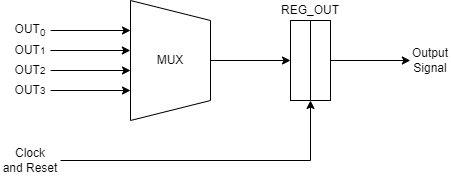
\includegraphics[width=0.7\textwidth]{img/Chapter2/OutputNetwork.png}
    \caption{Output Network}
    \label{fig:OutputNetwork}
\end{figure}

For this last network \textbf{one multiplexer} and \textbf{one register} are needed.